\documentclass[border=10pt]{standalone}
\usepackage[T1]{fontenc}
\usepackage{lmodern}
\usepackage{tikz}
\usetikzlibrary{shapes.geometric, arrows.meta, positioning, calc}

\definecolor{flblue}{HTML}{2c5f8a}
\definecolor{flbluebg}{HTML}{e8eef4}
\definecolor{outgreen}{HTML}{5a8a5a}
\definecolor{outgreenbg}{HTML}{e8f4e8}
\definecolor{muted}{HTML}{999999}

\begin{document}
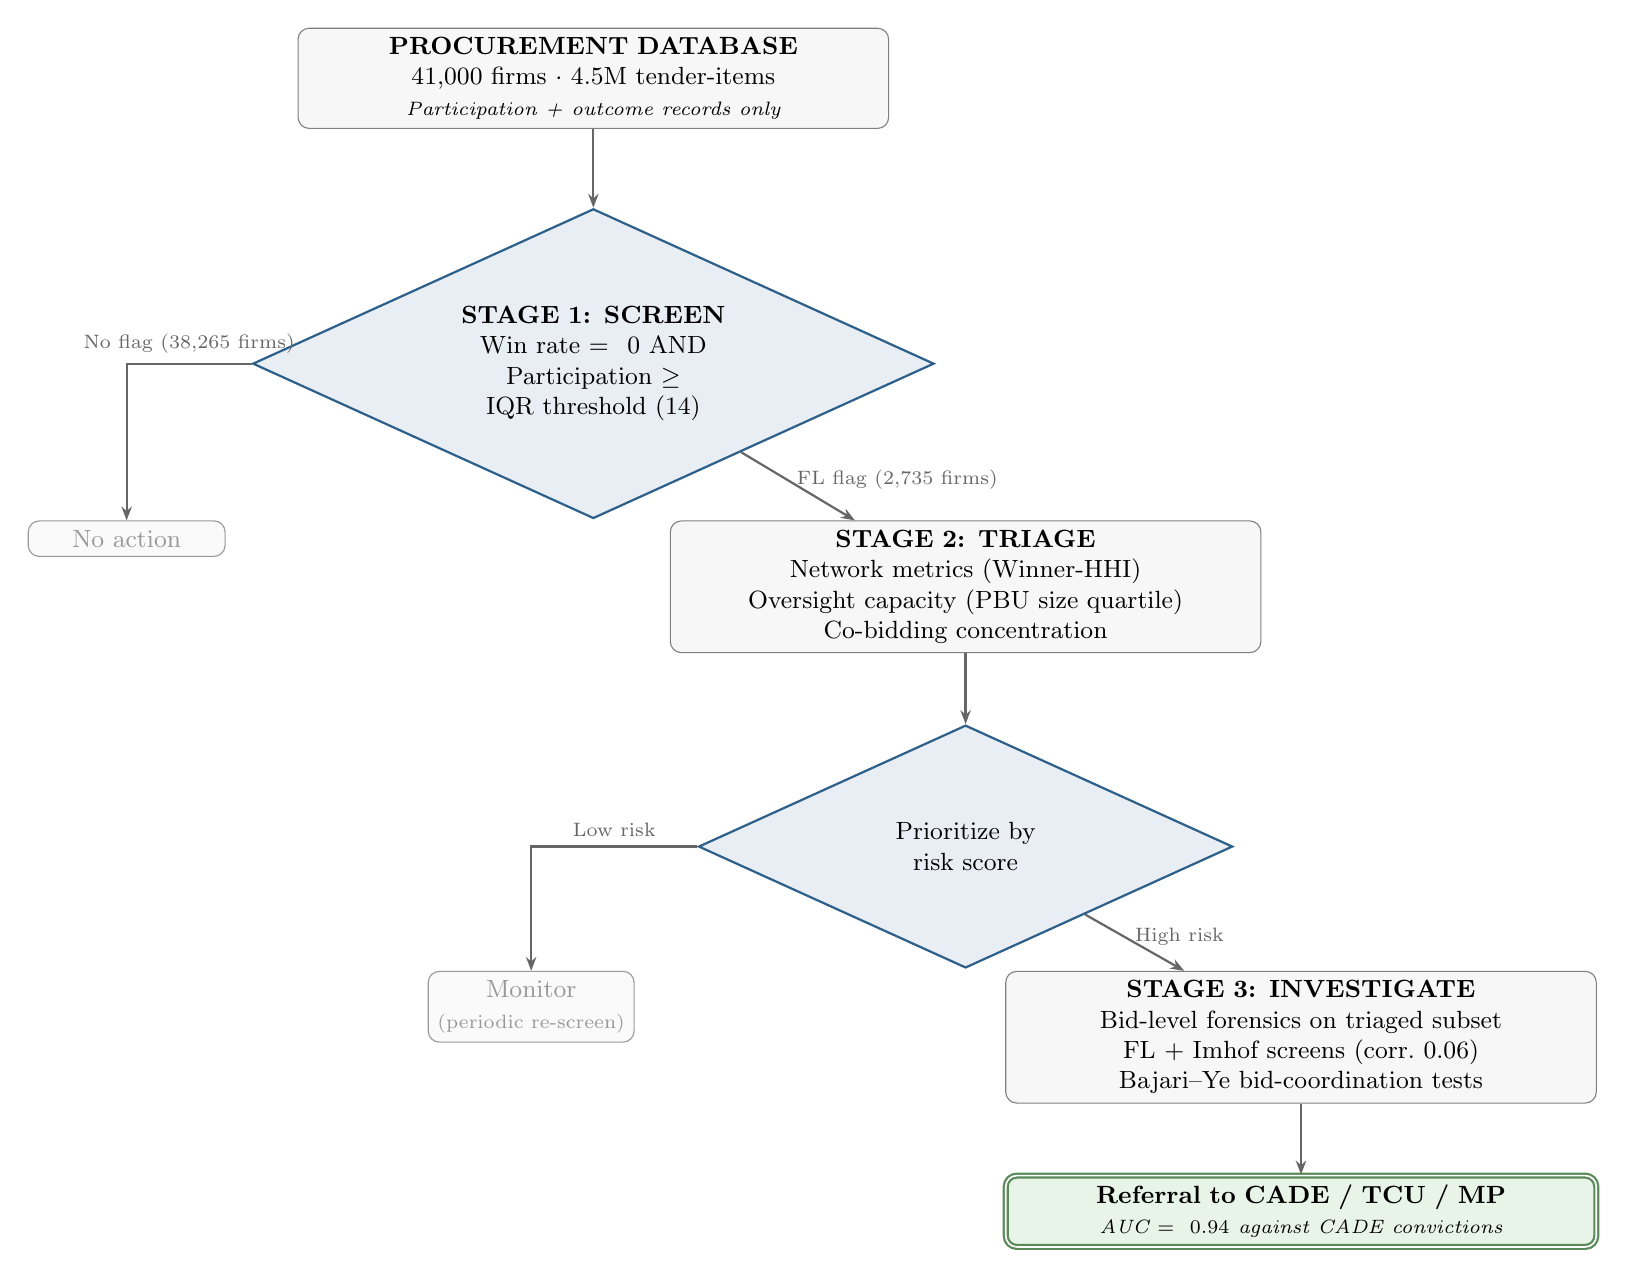
\begin{tikzpicture}[
    node distance=0.9cm and 1.5cm,
    every node/.style={font=\small, align=center},
    process/.style={rectangle, rounded corners=4pt, draw=black!50,
                    fill=black!3, minimum width=7.5cm, minimum height=1.1cm,
                    text width=7cm},
    decision/.style={diamond, draw=flblue, fill=flbluebg, thick,
                     minimum width=3cm, inner sep=2pt, text width=5cm,
                     aspect=2.2},
    output/.style={rectangle, rounded corners=4pt, draw=outgreen, fill=outgreenbg,
                   thick, double, minimum width=7.5cm, minimum height=0.9cm,
                   text width=7cm},
    noaction/.style={rectangle, rounded corners=4pt, draw=muted, fill=black!2,
                     text=muted, minimum width=2.5cm},
    arr/.style={-{Stealth[length=5pt]}, thick, color=black!60},
    lab/.style={font=\scriptsize, text=black!60}
]

% Nodes
\node[process] (db)
    {\textbf{PROCUREMENT DATABASE}\\
     41,000 firms $\cdot$ 4.5M tender-items\\
     {\scriptsize\itshape Participation + outcome records only}};

\node[decision, below=1.0cm of db] (screen)
    {\textbf{STAGE 1: SCREEN}\\
     Win rate $= 0$ AND\\
     Participation $\geq$ IQR threshold (14)};

\node[noaction, below left=1.0cm and 2.5cm of screen] (noflag)
    {No action};

\node[process, below right=1.0cm and -1.2cm of screen] (triage)
    {\textbf{STAGE 2: TRIAGE}\\
     Network metrics (Winner-HHI)\\
     Oversight capacity (PBU size quartile)\\
     Co-bidding concentration};

\node[decision, below=0.9cm of triage] (prio)
    {Prioritize by\\risk score};

\node[noaction, below left=0.8cm and 2.5cm of prio] (monitor)
    {Monitor\\{\scriptsize(periodic re-screen)}};

\node[process, below right=0.8cm and -1.2cm of prio] (invest)
    {\textbf{STAGE 3: INVESTIGATE}\\
     Bid-level forensics on triaged subset\\
     FL + Imhof screens (corr.\ 0.06)\\
     Bajari--Ye bid-coordination tests};

\node[output, below=0.9cm of invest] (refer)
    {\textbf{Referral to CADE / TCU / MP}\\
     {\scriptsize\itshape AUC $= 0.94$ against CADE convictions}};

% Arrows
\draw[arr] (db) -- (screen);
\draw[arr] (screen) -| node[lab, pos=0.25, above] {No flag (38,265 firms)} (noflag);
\draw[arr] (screen) -- node[lab, right, pos=0.4] {FL flag (2,735 firms)} (triage);
\draw[arr] (triage) -- (prio);
\draw[arr] (prio) -| node[lab, pos=0.25, above] {Low risk} (monitor);
\draw[arr] (prio) -- node[lab, right, pos=0.4] {High risk} (invest);
\draw[arr] (invest) -- (refer);

\end{tikzpicture}
\end{document}

